
In \fref{chap:intro} I have argued that the use of the MMSE in a filtering problem is an appropriate measure for the quality of a neural encoder. In this chapter I
will consider a number of examples, focusing especially on the case of dense populations of Gauss-Poisson neurons. In this case I will look at a general class of
linear stochastic processes described in \fref{chap:filtering,chap:mmse} and will consider the dependence of the MMSE for those processes in the encoder's 
parameters. In the case of dense populations of Gauss-Poisson neurons it makes the most sense to consider the width of the tuning functions as the central parameter 
of the encoder, which will be explained below. It is found that in general for this type of population of neurons there is a finite optimal tuning width which minimises the
MMSE of the filtering problem.\par

Following the investigation, I also present an analysis of dense populations of Gauss-Poisson neurons coding for more complex stochastic processes, such as bistable
processes. In this case, the filtering equations cease to be Gaussian, and we are forced to use approximate filtering approaches to obtain estimates of the MMSE.
I have used both the ADF approach with a Gaussian density and a simple particle filter and show results for these cases, which still show a finite width which minimises
the MMSE.\par

\section{Filtering through Point Processes and Optimal Codes}

Though we have introduced the general picture in \fref{chap:filtering}, I will shortly contextualise the framework again. As has been introduced, we are observing spike
trains from a population of neurons $N^i(t)$, whose rates depends on a stochastic process $X(t)$. Our objective is to estimate the state $X(t)$ from the observations
$\boldsymbol{N} = \{N^i(t)\}$ as precisely as possible. Let us denote the parameters of the encoder by $\varphi$.\footnote{In the case of our Gauss-Poisson neurons, we 
would have
$\varphi = \{\{\theta_i\}, \covar, \phi\}$.} Our optimal encoder would then be the encoder that minimises the MMSE, or more precisely
\begin{align*}
\varphi^* =& \argmin_\varphi \boldsymbol{E}\left[\Tr\left[\left(X(t) - \hat{X}(\boldsymbol{N}_{[t_0:t]})\right)\left(X(t) - \hat{X}(\boldsymbol{N}_{[t_0:t]})\right)^\top \right]\middle| X, \boldsymbol{N},\varphi\right]\\
=& \argmin_\varphi \Tr\left[\epsilon(\varphi)\right].
\end{align*}
Note that differently from \fref{chap:mss} we are considering the trace of the MMSE matrix here. This is frequently done to obtain a scalar measure of the quality of a
multidimensional estimation problem. The trace gives us the sum of the eigenvalues of the MMSE matrix, providing a practical measure of how far from the true value
the estimator is on average. Note also that in the second line I have dropped the time dependence as we will be mostly considering equilibrium results for the MMSE.
\par

\begin{figure}
\label{fig:filtering_expl}
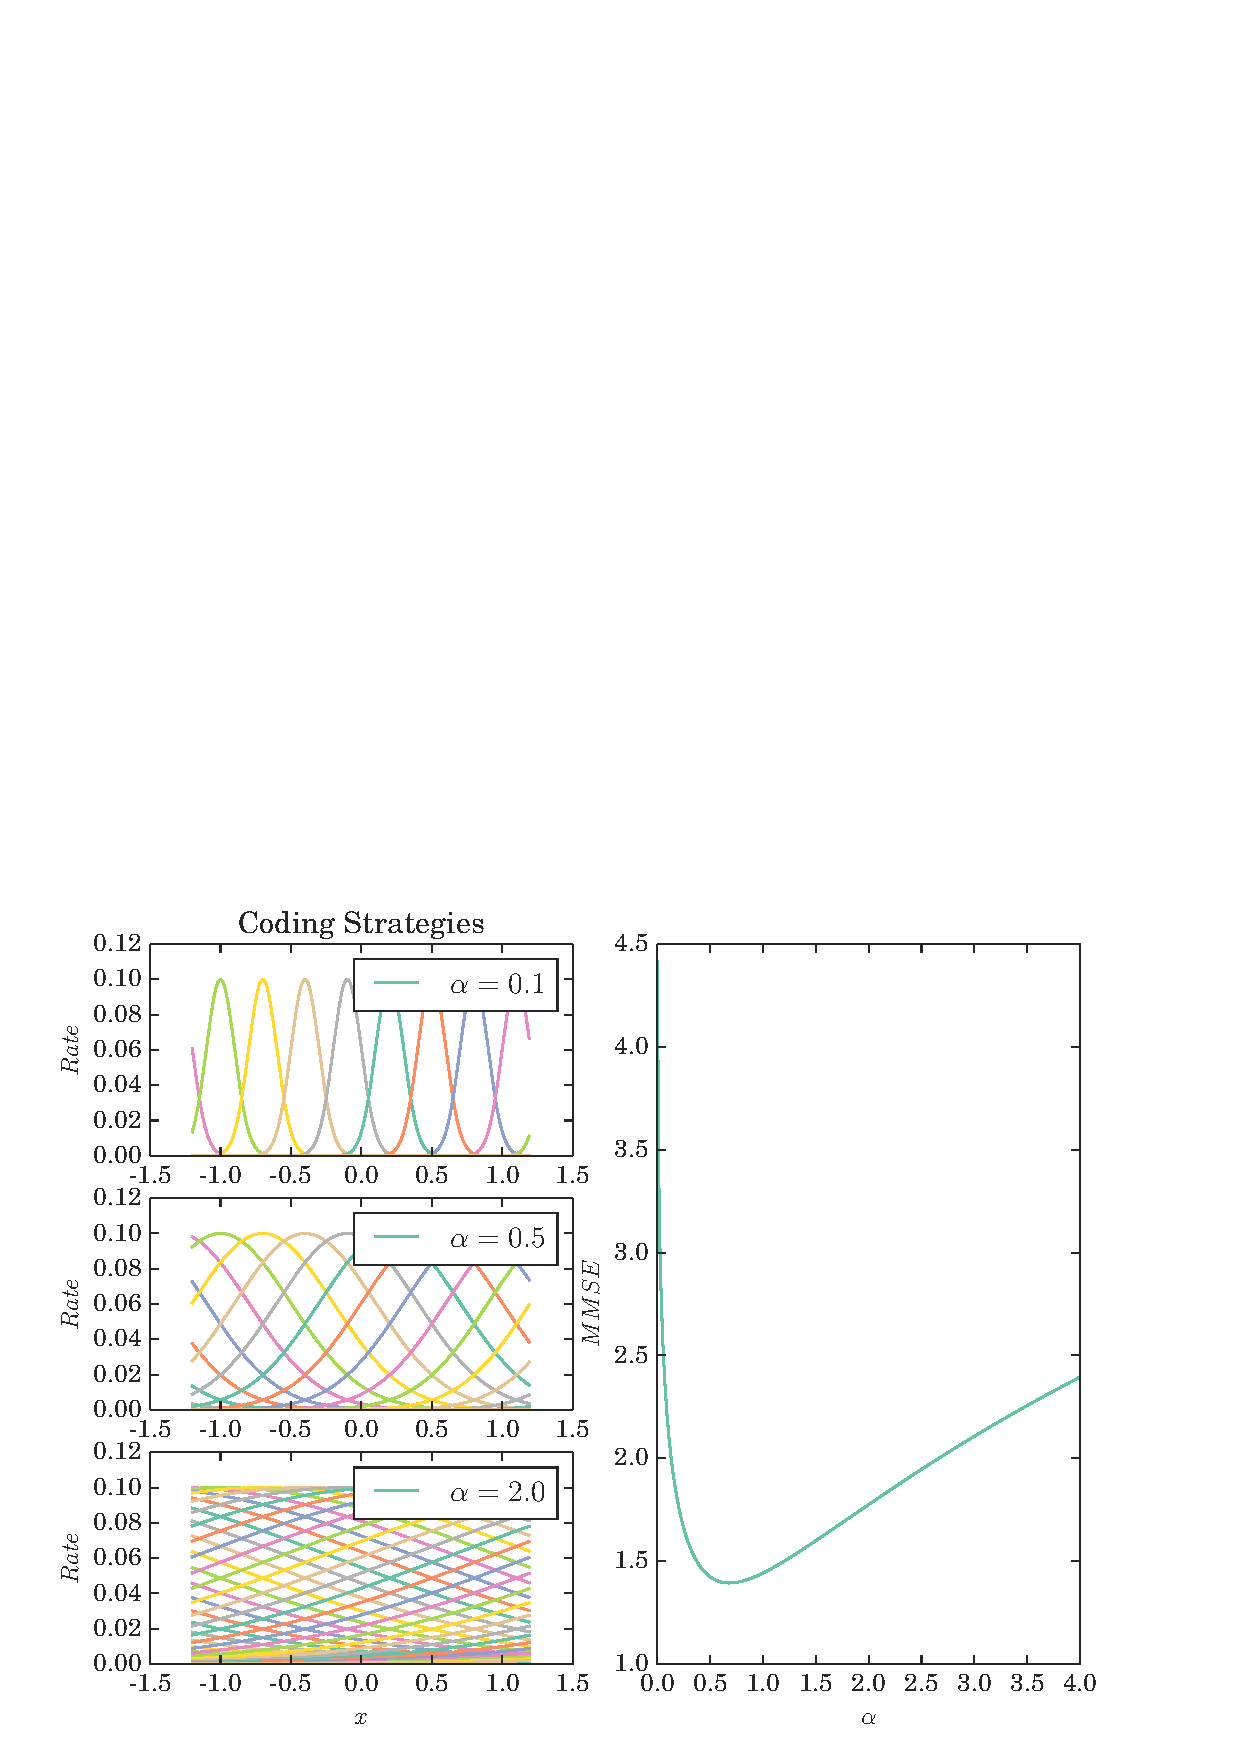
\includegraphics[width=\columnwidth]{figures/figure_5_1.png}
\caption{Optimal coding for filtering Problems: The leftmost column shows the tuning curves of the neurons in the population. Meanwhile, the middle column
shows the general setup of the filtering scheme for each population for the same stochastic process. Note the different situations for narrow and broad tuning curves.
The rightmost plot shows the MMSE as a function of the tuning width $\alpha$.}
\end{figure}

\subsection{Optimal Codes for Control}

In \fref{chap:control} I have introduced the formalism of stochastic optimal control and shown how to extend it to deal with point process observations. In the same way
as one can define an optimal encoder for a filtering problem, one can define an optimal encoder for a control problem. Given a control problem with a cost function given
by
\[
C(\boldsymbol{N}_{[0,T]},U_{[0,T]}) =\boldsymbol{E}\left[ \int_0^T c(X(t),U(\boldsymbol{N}_{[0,t]})) dt\middle| \boldsymbol{N}\right],
\]
we can like above define the optimal encoder to be the one with parameter $\varphi^*$ given by
\[
\varphi^* = \argmin_\varphi C(\boldsymbol{N}_{[0,T]},U_{[0,T]};\varphi).
\]
These can lead to different results than the filtering framework as has been shown in \cite{Susemihl2014}.

\section{Filtering Linear Stochastic Processes through dense Gauss-Poisson Spike Trains}

Let us then consider a linear stochastic process of the type
\[
dX(t) = AX(t) + H^{1/2} dW(t).
\]
Though this may seem as a somewhat restrictive choice, note that a number of processes can be cast into this format. The simple OU process, which I considered in
\fref{chap:mss} is one example, but generalisations to higher dimensions are relatively simple and include, for example, the stochastic damped oscillator. Taking
the matrices
\[
A= \left(\begin{array}{cc} 0 & 1\\ -\omega^2&-\gamma\end{array}\right), \textrm{ and }H= \left(\begin{array}{cc} 0 & 0\\ 0& \eta \end{array}\right),
\]
will lead to a stochastic process with a periodic component. In \fref{fig:stoch_example} a few examples of linear stochastic systems are shown, with a couple of 
samples of each per plot. Note that, although the focus here is on stationary stochastic processes, for which the distribution converges in the limit of long times,
this is by no means a necessity for the analysis at hand. Even for non-stationary processes such as the Wiener process,\marginnote{The Wiener process $W(t)$ has
a covariance that increases linearly with time.} the posterior density can be stationary, allowing us to evaluate the equilibrium MMSE.\par

\begin{figure}
\label{fig:filtering_expl}
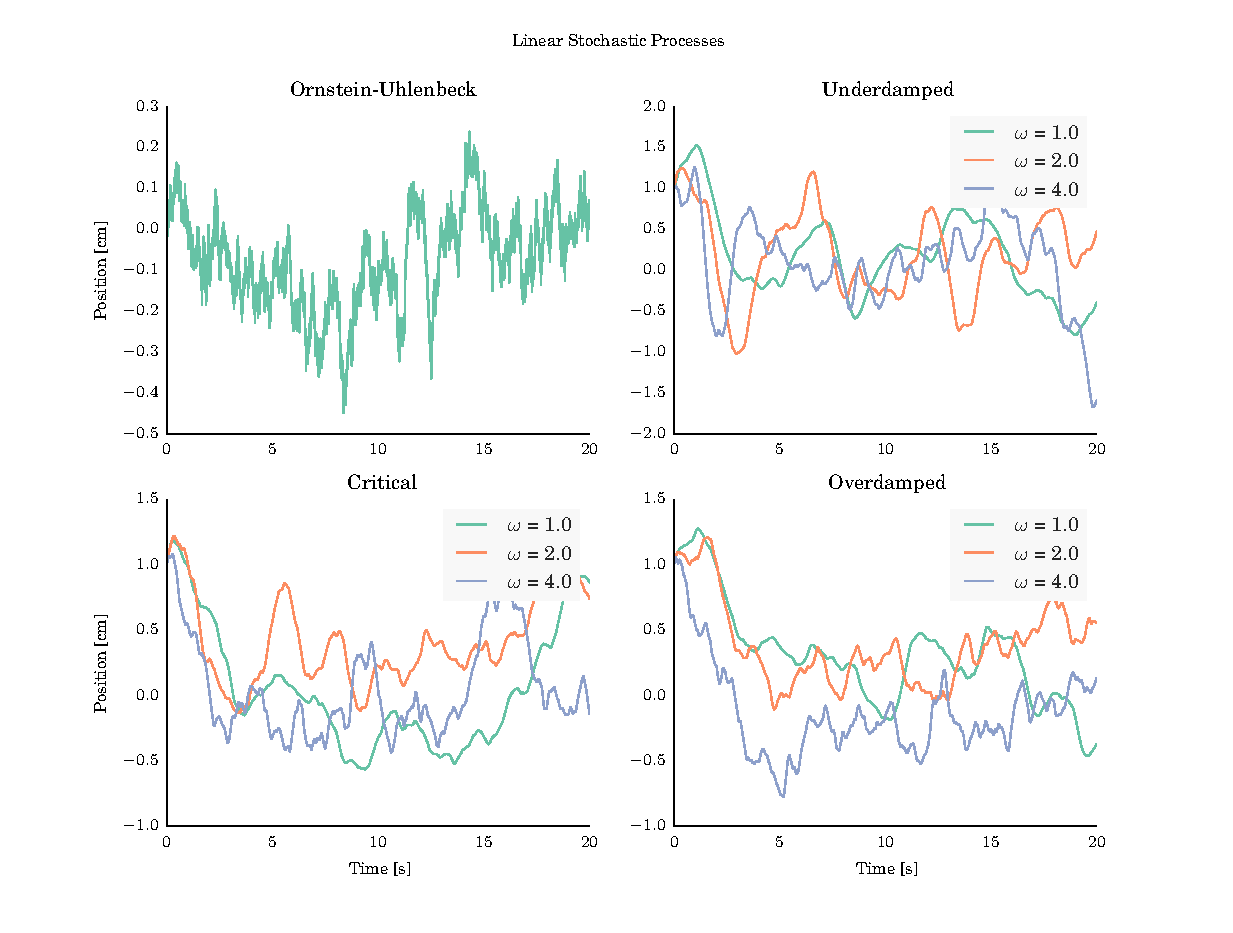
\includegraphics[width=\columnwidth]{figures/figure_5_2.eps}
\caption{Linear stochastic processes: From the top left, we have the one-dimensional Ornstein-Uhlenbeck process, an underdamped stochastic oscillator,
a critically damped stochastic oscillator (bottom left), and an over damped stochastic oscillator.}
\end{figure}


The MMSE $\epsilon(t)$ can then be obtained from the formalism derived in \fref{chap:mse}. Throughout this section I will refer to both the numerical solution of the
evolution equations for $\epsilon(t)$ as well as the mean-field approximation to it. Let me start with the simplest stochastic process, the Ornstein-Uhlenbeck process
given by
\[
dX(t) = -\gamma X(t) dt + \sigma^{1/2} dW(t),
\]
where the evolution of the MMSE is given by
\[
\frac{d\epsilon(t)}{dt} = -2\gamma \epsilon(t) + \sigma -\hat{\lambda} \boldsymbol{E}\left[\frac{s^2}{\alpha^2+s}\right].
\]
We can now consider the temporal evolution of the MMSE, as it has been shown in \fref{fig:matern_coding} for a Matern process. 
We will focus on the equilibrium value of the MMSE, that is, we will focus on the long-term performance of the encoder in the filtering problem, rather than focusing
on the transient, short-time behaviour. Below in \fref{fig:encoder_OU} we can see the equilibrium MMSE of a dense Gauss-Poisson population of neurons encoding
an OU process. The dependence on both the maximal firing rate $\phi$ and the tuning width $\alpha$ is shown.

\begin{figure}
\label{fig:mmse_ou}
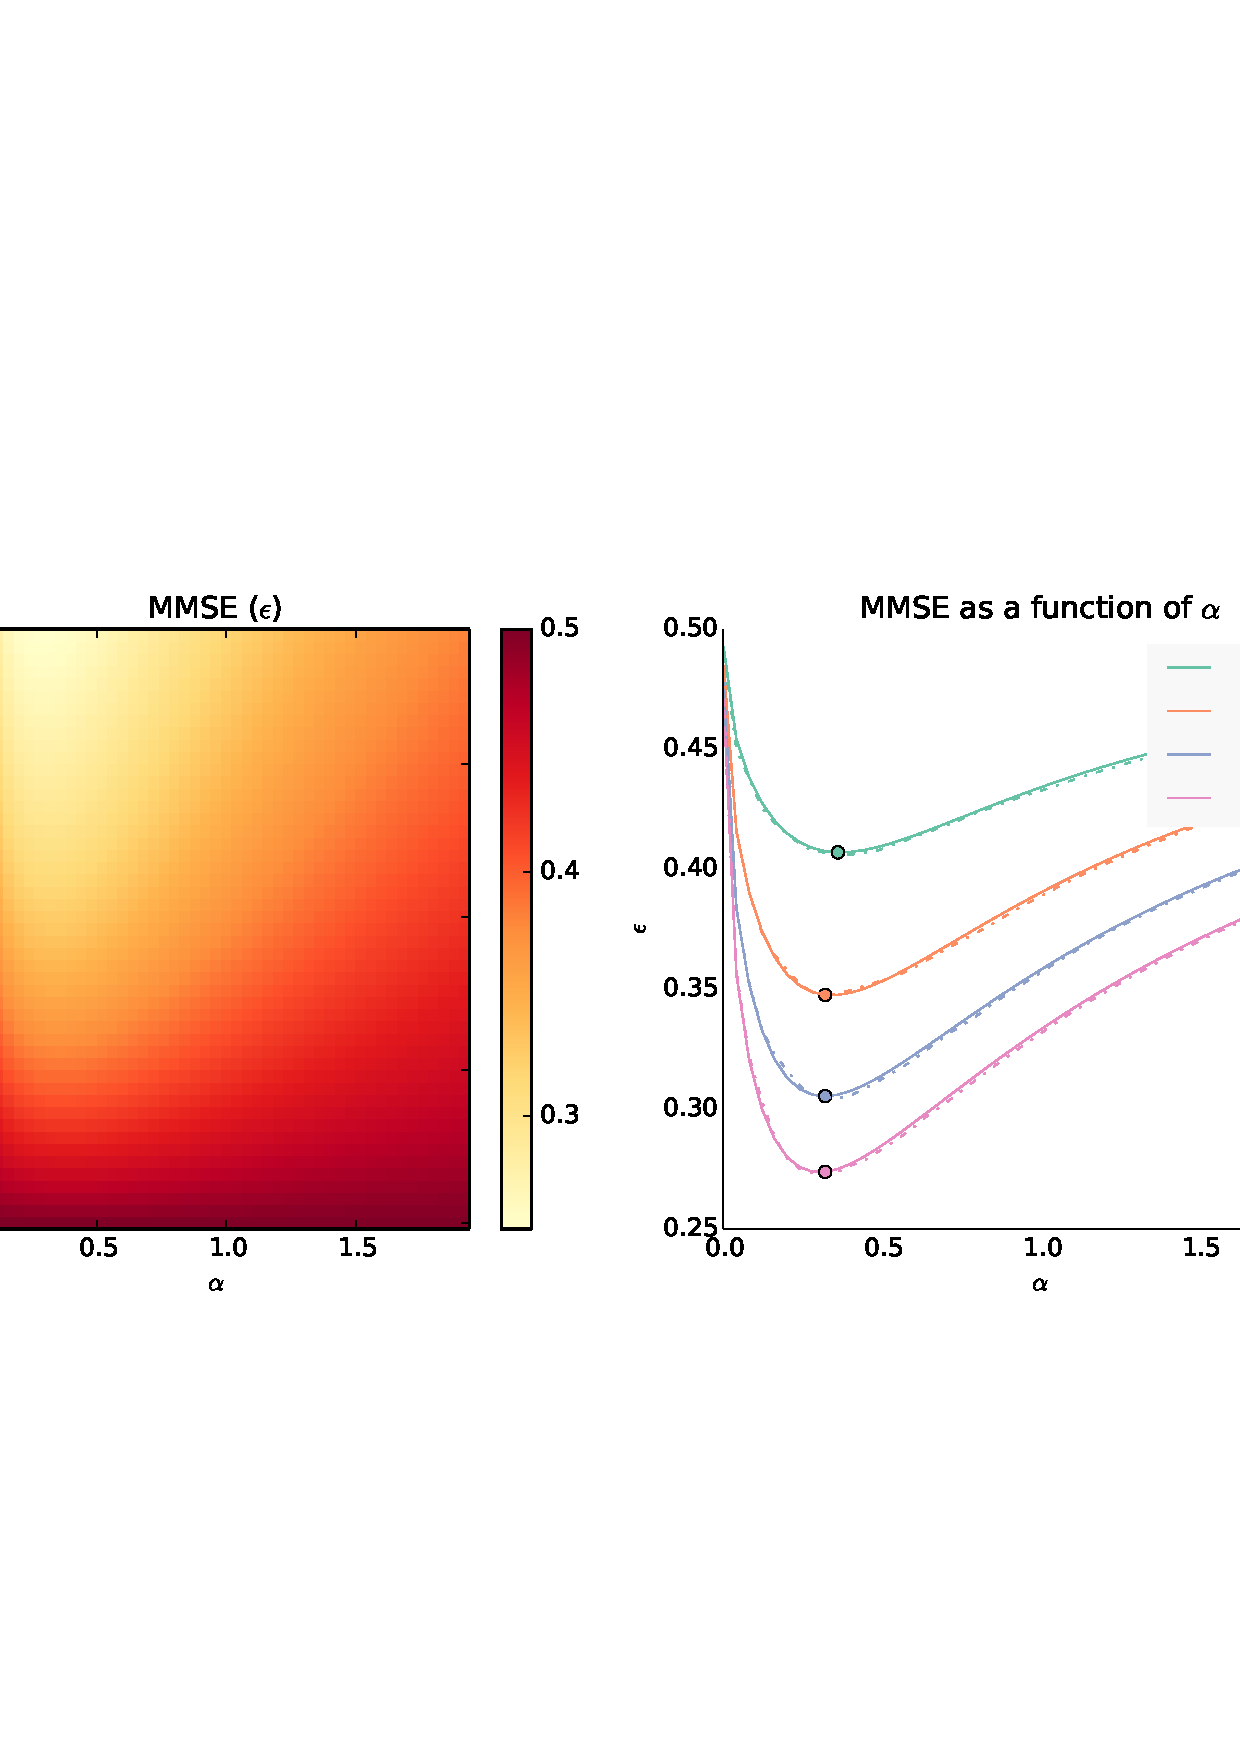
\includegraphics[width=\columnwidth]{figures/figure_5_3.png}
\caption{Comparing Encoders for Filtering: The left hand panel shows a heat map of the MMSE as a function of the maximal firing rate $\phi$ and the tuning
width $\alpha$. There is a trade-off between the number of spikes and the precision of the spikes, manifesting itself in a finite tuning width that minimises the
the MMSE. For any $\alpha$ increasing the firing rate $\phi$ simply decreases the MMSE. The right panel shows the dependence in $\alpha$ for a few values
of $\phi$.}
\end{figure}

More interestingly, we can now ask ourselves how the optimal encoder depends on any of the parameters of the problem. Let us say the parameter $\gamma$
which defines the time-scale of correlations in the OU process.\footnote{Remember that the prior kernel of the OU process is given by $k(s,t) = \frac{\eta^2}{2\gamma} \exp(-\frac{|s-t|}{2\gamma}$.} In \fref{fig:ecological_OU} I have plotted the optimal encoding width $\alpha^*$ as a function of $\gamma$, $\sigma$ and
$\phi$. Though the results are not entirely unexpected, it is interesting to be able to provide an accurate account of the ecological dependence of the optimal 
encoder. Shorter time-scales (larger values of $\gamma$) require a higher frequency of spikes, as the information conveyed by those spikes becomes irrelevant
more quickly. Thus, holding the maximal firing rate $\phi$ fixed, the way to increase the frequency of spikes is to have broader tuning functions. So, as $\gamma$
increases, so does $\alpha^*$.

\begin{figure}
\label{fig:mmse_ou}
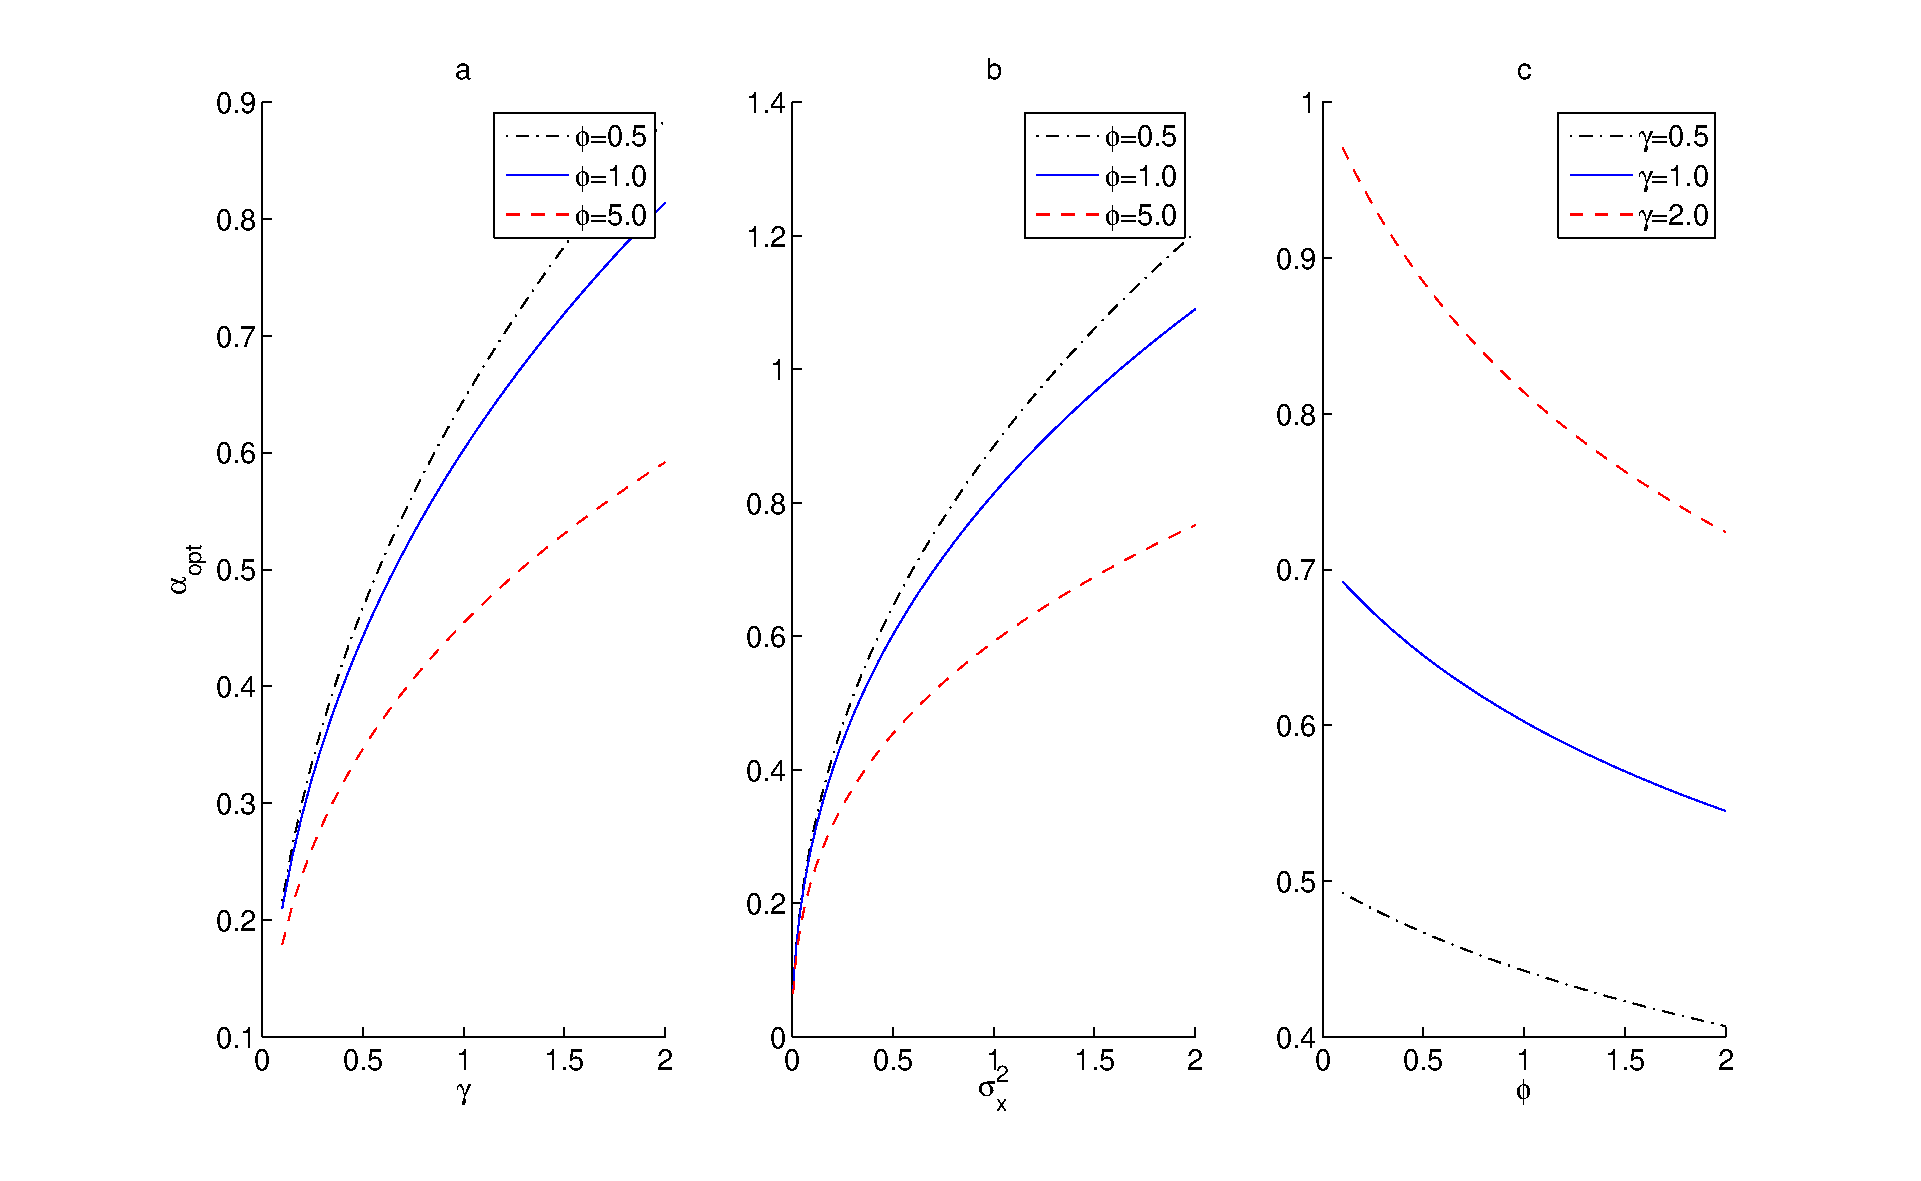
\includegraphics[width=\columnwidth]{figures/figure_5_4.eps}
\caption{Ecological Dependence of the Optimal Encoder:}
\end{figure}

\section{Mean-Field Approach}

\section{Analytic Approaches}

\section{Performance Measures}
